\documentclass[12pt,a4paper]{article}

% Essential packages
\usepackage[utf8]{inputenc}
\usepackage[T1]{fontenc}
\usepackage{amsmath,amsfonts,amssymb}
\usepackage{graphicx}
\usepackage{float}
\usepackage{cite}
\usepackage{url}
\usepackage{hyperref}
\usepackage{geometry}
\usepackage{setspace}
\usepackage{titlesec}
\usepackage{caption}
\usepackage{subcaption}
\usepackage{booktabs}
\usepackage{siunitx}
\usepackage{lineno}
\usepackage[utf8]{inputenc}
\usepackage{tikz}
\usepackage{tikz-qtree}
\usetikzlibrary{trees}


\setcounter{secnumdepth}{5}  % Numbers down to paragraph level
\setcounter{tocdepth}{5}  

% Page setup
\geometry{
    a4paper,
    margin=2.5cm,
    top=3cm,
    bottom=3cm
}

% Line spacing
\doublespacing

% Line numbers (uncomment if required by journal)
% \linenumbers

% Section formatting
\titleformat{\section}{\large\bfseries}{\thesection.}{1em}{}
\titleformat{\subsection}{\normalsize\bfseries}{\thesubsection.}{1em}{}

% Figure and table captions
\captionsetup{font=small,labelfont=bf}

% Hyperlink setup
\hypersetup{
    colorlinks=true,
    linkcolor=black,
    citecolor=blue,
    urlcolor=blue
}

% Title page information
\title{\textbf{Time-variant kinetics: a Framework for Microbial Impacts on Soil Organic Carbon Decomposition}}

\author{
    First Author\textsuperscript{1,2}*, 
    Second Author\textsuperscript{1}, 
    Third Author\textsuperscript{3}\\
    ...\textsuperscript{4}\\
    \\
    \textsuperscript{1}Department of [Department], [University Name], [City, Country]\\
    \textsuperscript{2}[Second Affiliation if applicable]\\
    \textsuperscript{3}[Third Institution]\\
    \textsuperscript{4}[...]\\
    \\
    *Corresponding author: email@institution.edu
}

\date{}


% In preamble
\newenvironment{graphicalabstract}{%
  \section*{Graphical Abstract}
  \begin{center}
}{%
  \end{center}
}



\begin{document}

\maketitle

\begin{abstract}
\noindent

Here something to add at the end

\textbf{Keywords:} keyword1, keyword2, keyword3, keyword4, keyword5
\end{abstract}

\newpage


\begin{graphicalabstract}

\begin{figure}[htbp]
\centering
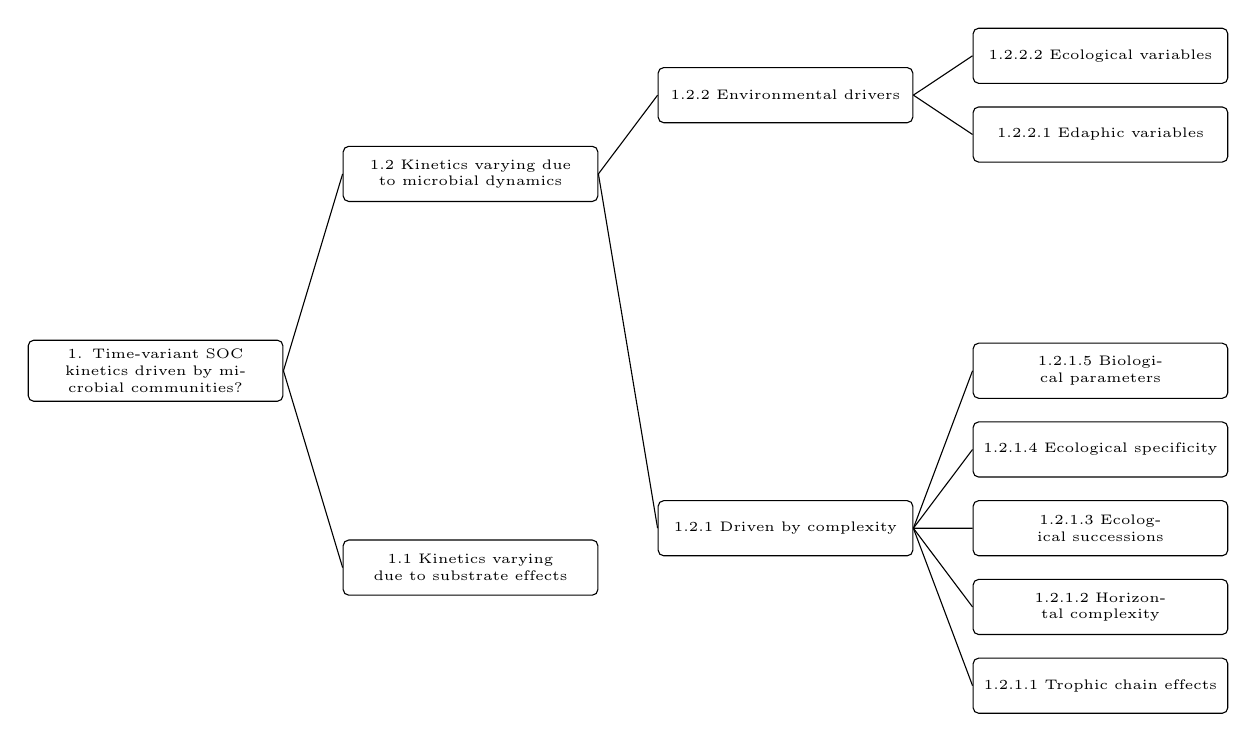
\begin{tikzpicture}[
  grow=right,
  level 1/.style={sibling distance=5cm, level distance=4cm},
  level 2/.style={sibling distance=2cm, level distance=4cm},
  level 3/.style={sibling distance=1cm, level distance=4cm},
  level 4/.style={sibling distance=1cm, level distance=4cm},
  every node/.style={draw, rectangle, rounded corners=2pt, 
                     minimum height=0.7cm, text width=3cm, 
                     align=center, font=\tiny}
]

\node {1. Time-variant SOC kinetics driven by microbial communities?}
  child {
    node {1.1 Kinetics varying due to substrate effects}
  }
  child {
    node {1.2 Kinetics varying due to microbial dynamics}
    child [yshift=-3.5cm] {
      node {1.2.1 Driven by complexity}
      child {
        node {1.2.1.1 Trophic chain effects}
      }
      child {
        node {1.2.1.2 Horizontal complexity}
      }
      child {
        node {1.2.1.3 Ecological successions}
      }
      child {
        node {1.2.1.4 Ecological specificity}
      }
      child {
        node {1.2.1.5 Biological parameters}
      }
    }
    child {
      node {1.2.2 Environmental drivers}
      child {
        node {1.2.2.1 Edaphic variables}
      }
      child {
        node {1.2.2.2 Ecological variables}
      }
    }
  };

\end{tikzpicture}
\caption{Hierarchical framework for variable kinetics in soil organic carbon models. The framework distinguishes between substrate-driven (1.1) and microbial-driven (1.2) mechanisms, with microbial dynamics further categorized by complexity factors and environmental drivers.}
\label{fig:kinetics_framework}
\end{figure}

\end{graphicalabstract}


% Optional: page with table of content, useful during writing
\tableofcontents
\newpage  

\section{Introduction} \label{sec:intro}


\subsection{The SOC Modeling Challenge} \label{sec:intro_challenge}

Current state of SOC models in production use, limitations of 2-3 decade old constant kinetics assumptions, and why variable kinetics matter for climate projections.

\subsection{From First-Order to Higher-Order Kinetics} \label{sec:intro_kinetics}

Historical development of SOC kinetic models, chemical vs. biological controls on decomposition, and the role of microbial communities in kinetic complexity.

\subsection{Scope and Objectives} \label{sec:intro_scope}

Framework for organizing variable kinetics mechanisms, integration of spatial and temporal variability, research gaps and future directions.


\section{Theoretical Background: Kinetic Models in Soil Carbon Cycling} \label{sec:theory}

\subsection{Classical First-Order Kinetics} \label{sec:theory_first}

Mathematical foundations, assumptions and limitations, and why they persist in production models.

\subsection{Higher-Order Kinetic Models} \label{sec:theory_higher}

Michaelis-Menten and enzyme kinetics, regulatory mechanisms and feedback loops, examples from Schimel \& Weintraub (2003) and predecessors.

\subsection{Spatial and Temporal Heterogeneity} \label{sec:theory_heterogeneity}

Scale-dependent processes and linking molecular to ecosystem scales.


\section{Substrate-Driven Variable Kinetics} \label{sec:substrate}

\subsection{Priming Effects and SOC Quality} \label{sec:substrate_priming}

Classical priming hypotheses, spatial variations in substrate availability, and connections between quality and kinetic parameters.

\subsection{Substrate Heterogeneity Across Landscapes} \label{sec:substrate_landscape}

Chemical composition gradients, physical protection mechanisms, and implications for model parameterization.




\section{Microbial-Driven Variable Kinetics: The Complexity Framework} \label{sec:microbial}


\subsection{Complexity-Driven Dynamics} \label{sec:microbial_complexity}


\subsubsection{Vertical Complexity: Trophic Chain Effects} \label{sec:microbial_vertical}

Predator-prey dynamics in soil food webs, mesofauna and microfauna influences, isotopic fractionation as complexity indicators, and case studies of accelerated C cycling in complex systems.


\subsubsection{Horizontal Complexity: Synergistic Associations} \label{sec:microbial_horizontal}

Enzyme complementarity and synergies, diversity-function relationships, applications to degraded soils, and synthetic community experiments.


\subsubsection{Temporal Dynamics: Ecological Successions} \label{sec:microbial_succession}

Mycorrhizal succession patterns, forest stand development and C cycling, sink/source transitions over decades, and case study of Cortinarius succession.


\subsubsection{Spatial Specificity: Local Adaptation} \label{sec:microbial_specificity}

Field Advantage hypothesis, home-field advantage effects, and geographic and climatic controls.


\subsubsection{Intrinsic Microbial Biological Parameters} \label{sec:microbial_intrinsic}

Carbon use efficiency (CUE) variability, physiological constraints, and trade-offs and optimization.


\subsection{Environmental Drivers} \label{sec:microbial_environment}

\subsubsection{Edaphic Controls} \label{sec:microbial_edaphic}

Soil physical and chemical properties, persistent landscape effects, and spatial modeling implications.

\subsubsection{Above-Belowground Linkages} \label{sec:microbial_linkages}

Plant-soil feedbacks, seasonal and phenological controls, cross-ecosystem comparisons.


\subsection{Variable climate forcing: can temperature and moisture sensitivities of SOC decomposition be community-driven?} \label{sec:variable_forcing}


\section{The abiotic gate hypothesis and its possible linkages}


\section{Synthesis and Integration} \label{sec:synthesis}

\subsection{Unified Framework for Variable Kinetics} \label{sec:synthesis_framework}

Hierarchical organization of mechanisms, interactions between substrate and microbial drivers, and scale-dependent relative importance.
This could be a D.A.G formulation of the plot in the graphical abstract with maybe a bit more detail


\subsection{Implications for Model Development} \label{sec:synthesis_models}

Testing toy models here

\subsubsection{ Hyp 1 model implications}

\subsubsection{ Hyp ... model implications}


\subsection{Knowledge gap: bridging scales in modeling} \label{sec:synthesis_scales}

Problems of upscaling, including uncertainty issues


\section{Current Research Frontiers and Future Directions} \label{sec:future}

\subsection{Methodological Advances} \label{sec:future_methods}

Multi-omics approaches, isotopic techniques and fractionation studies, and long-term experimental platforms.

\subsection{Emerging Concepts} \label{sec:future_concepts}

Network ecology in soil systems, machine learning applications, and climate change adaptation mechanisms.

\subsection{Research Priorities} \label{sec:future_priorities}

Critical knowledge gaps, experimental design considerations, and model-data integration needs.


\section{Conclusions} \label{sec:conclusions}

\subsection{Key Insights} \label{sec:conclusions_insights}

Summary of variable kinetics mechanisms, relative importance under different conditions, and implications for current model limitations.

\subsection{Toward Next-Generation SOC Models} \label{sec:conclusions_models}

Essential features for new model frameworks, implementation pathways, and expected improvements in predictive capacity.




\section*{Acknowledgments}

Not sure here but we will probably have to acknowledge quite some people and institutions

\section*{Funding}

We should have a few, I guess.

\section*{Conflicts of Interest}

The authors declare no conflicts of interest.


\section*{Data Availability Statement}

Not sure we will need it.



\section{References}
We need to use bibtex here!


\end{document}